%==============================================================================
%  THE LEDGER — Distributor Credit Risk Engine
%  Technical Report · skillSYNC (a skillit company) · Pair B
%  Compile with pdfLaTeX on Overleaf.
%==============================================================================
\documentclass[11pt,a4paper]{article}

\usepackage[T1]{fontenc}
\usepackage[utf8]{inputenc}
\usepackage{charter}
\usepackage[scaled=0.92]{helvet}
\usepackage[margin=2.2cm,top=2.4cm,bottom=2.2cm]{geometry}
\usepackage{xcolor}
\usepackage{tikz}
\usepackage{booktabs}
\usepackage{colortbl}
\usepackage{tabularx}
\usepackage{array}
\usepackage{enumitem}
\usepackage{titlesec}
\usepackage[most]{tcolorbox}
\usepackage{fancyhdr}
\usepackage{microtype}
\usepackage{ragged2e}
\usepackage[hidelinks]{hyperref}

%------------------------------- palette --------------------------------------
\definecolor{navy}{HTML}{1E2761}
\definecolor{navydeep}{HTML}{14193F}
\definecolor{gold}{HTML}{C9A24B}
\definecolor{goldpale}{HTML}{F0E6CC}
\definecolor{ice}{HTML}{CADCFC}
\definecolor{parch}{HTML}{F7F4EE}
\definecolor{ink}{HTML}{1A1A2E}
\definecolor{slate}{HTML}{5A5A72}
\definecolor{rulec}{HTML}{DDD6C8}
\definecolor{ok}{HTML}{1E7A44}
\definecolor{warn}{HTML}{A97318}
\definecolor{bad}{HTML}{B3392C}

\color{ink}
\setlength{\parskip}{5pt}
\setlength{\parindent}{0pt}
\renewcommand{\arraystretch}{1.28}

%------------------------------- headings -------------------------------------
\titleformat{\section}
  {\normalfont\Large\bfseries\color{navy}}
  {\color{gold}\thesection}{0.7em}{}
\titlespacing*{\section}{0pt}{16pt}{6pt}

\titleformat{\subsection}
  {\normalfont\large\bfseries\color{navy}}
  {\color{gold}\thesubsection}{0.6em}{}
\titlespacing*{\subsection}{0pt}{12pt}{4pt}

%------------------------------- headers --------------------------------------
\pagestyle{fancy}
\fancyhf{}
\renewcommand{\headrulewidth}{0.4pt}
\renewcommand{\headrule}{\hbox to\headwidth{\color{rulec}\leaders\hrule height \headrulewidth\hfill}}
\fancyhead[L]{\footnotesize\color{slate}The Ledger — Distributor Credit Risk Engine}
\fancyhead[R]{\footnotesize\color{slate}skillSYNC · Pair B}
\fancyfoot[C]{\footnotesize\color{slate}\thepage}

%------------------------------- helpers --------------------------------------
% Callout box
\newtcolorbox{callout}[1][]{
  colback=parch, colframe=rulec, boxrule=0.4pt, arc=2pt,
  left=8pt, right=8pt, top=6pt, bottom=6pt, #1}

% Highlight box (navy)
\newtcolorbox{keybox}[1][]{
  colback=navy, colframe=navy, boxrule=0pt, arc=2pt,
  coltext=white, left=10pt, right=10pt, top=7pt, bottom=7pt, #1}

% Small caps label
\newcommand{\lab}[1]{{\color{navy}\bfseries\footnotesize #1}}

% Stat callout
\newcommand{\stat}[3]{%
\begin{minipage}[t]{#1}
\raggedright
{\color{#3}\fontsize{20}{22}\selectfont\bfseries #2}
\end{minipage}}

\begin{document}

%==============================================================================
% TITLE PAGE
%==============================================================================
\begin{titlepage}

\begin{tikzpicture}[remember picture,overlay]
  \fill[navydeep] (current page.north west) rectangle (current page.south east);
  \foreach \i in {1,...,26}{
    \fill[gold,opacity=0.10]
      ([yshift=-\i*1.05cm]current page.north west) rectangle
      ([yshift=-\i*1.05cm-0.03cm]current page.north east);}
\end{tikzpicture}

\vspace*{4.6cm}
{\color{gold}\footnotesize\bfseries\sffamily
 DISTRIBUTOR CREDIT RISK \quad·\quad TECHNICAL REPORT}

\vspace{0.8cm}
{\color{white}\fontsize{40}{46}\selectfont\bfseries The Ledger}

\vspace{0.35cm}
{\color{ice}\fontsize{17}{22}\selectfont\itshape
 From gut feel to defensible data}

\vspace{1.1cm}
{\color{white}\normalsize
\begin{minipage}{0.82\textwidth}
\setlength{\parskip}{0pt}
A credit risk scoring engine that reads a distributor's own payment ledger and
returns an explainable 300--900 risk score for every dealer --- including the
accounts the sales team personally vouches for.
\end{minipage}}

\vspace{1.6cm}
{\color{gold}\rule{4.2cm}{1.1pt}}

\vspace{0.7cm}
{\color{white}\normalsize\bfseries skillSYNC} \;
{\color{ice}\normalsize a skillit company}

\vspace{0.35cm}
{\color{ice}\normalsize Pair B \;\textbar\; Abdul Ghafoor \;\textperiodcentered\; Ahmed Qureshi}

\vspace{0.2cm}
{\color{ice}\small AI/ML Engineering Track \;\textbar\; Problem 01}

\vfill
{\color{gold}\footnotesize
 Status: deployed and publicly accessible \quad·\quad
 Validated across six independent portfolios}
\vspace{1.5cm}
\end{titlepage}

%==============================================================================
\section*{Executive Summary}
\addcontentsline{toc}{section}{Executive Summary}
\vspace{-4pt}

Pakistani distribution houses extend trade credit to hundreds of dealers on the
strength of a salesman's personal judgement. There is no score, no structured
assessment, and no counterweight to a relationship. The cost is measurable:
industry sources place bad debt at 3--7\% of revenue, with PKR~1M+ written off
annually and over 100 hours a year spent chasing payments.

\textbf{The Ledger} converts a distributor's existing invoice history into a
defensible risk signal. It engineers six behavioural features grounded in
Pakistani trade practice, fits a Weight-of-Evidence logistic scorecard, and
returns a 300--900 score per dealer with plain-language reason codes, a ranked
risk table, and a downloadable memo for each account.

The system is deliberately built for the market it serves. It accepts the
column names, date formats and currency conventions a real ledger export
actually contains; it derives its own analysis window and its own definition of
``late'' from each portfolio; and where the shipped model is a poor fit, it
trains one on the uploaded data and cross-validates it before use. Critically,
it reports how far its own output can be trusted --- and declines to score
rather than producing confident numbers on unsuitable data.

\vspace{4pt}
\begin{keybox}
\textbf{Headline result.} Across three independently constructed portfolios with
known outcomes --- differing in schema, size, date range and payment culture ---
the system flagged \textbf{every genuinely risky dealer} for attention and
produced \textbf{zero false accusations}, with perfect risk ordering in all
three cases.
\end{keybox}

\begin{callout}
\lab{HONEST SCOPE.} All validation to date uses constructed portfolios with
embedded ground truth. No real-world dealer default has yet been observed. The
RED/AMBER/GREEN tier is the reliable signal; the exact numeric score is
directional. This limitation is stated throughout rather than deferred to a
footnote.
\end{callout}

%==============================================================================
\section{Problem Context}

\subsection{The decision as it is made today}

Credit is extended on a sentence: \emph{``yaar, acha banda hai --- de do.''}
The salesman vouches, the goods ship, and nobody consults the ledger. Three
structural forces sustain this:

\begin{itemize}[leftmargin=1.3em,itemsep=2pt,topsep=3pt]
  \item \textbf{Near-zero ERP adoption} in mid-tier distribution. Payment
        history exists, but scattered across Excel sheets and handwritten
        ledgers rather than a queryable database.
  \item \textbf{Relationship-based trust culture.} Refusing credit to a known
        counterparty carries social cost that a spreadsheet does not offset.
  \item \textbf{Misaligned incentives.} Salesmen earn commission on volume and
        bear no downside when a dealer they vouched for defaults.
\end{itemize}

The third point shapes the entire design. The feature currently driving
decisions --- salesman judgement --- is not merely uninformative; it is
\emph{adversarial} to the outcome being predicted. A useful system must
therefore be prepared to contradict the person who knows the dealer best, and
must justify itself when it does.

\subsection{Who this is for}

Owners of FMCG, pharmaceutical and textile distribution houses managing 50--500
dealers, together with the finance leads and 3--10 field salesmen operating
under them. These are businesses without a data team, without an ERP, and
without access to credit bureau coverage for the small retailers they supply.
Every design decision follows from that: the output must be readable by a
non-technical owner, and the input must be whatever their system already
produces.

%==============================================================================
\section{System Architecture}

The deliverable is a deployed web application, not a notebook.

\vspace{2pt}
\begin{center}
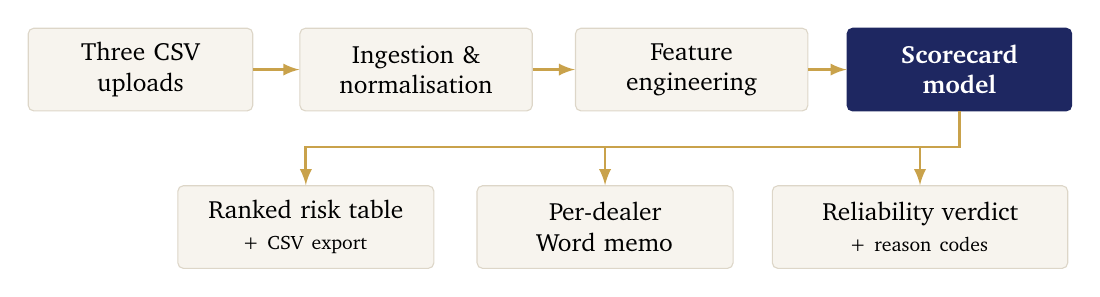
\begin{tikzpicture}[
  node distance=0pt,
  box/.style={draw=rulec, fill=parch, rounded corners=2pt, minimum height=1.05cm,
              align=center, font=\small, inner sep=5pt},
  nbox/.style={draw=navy, fill=navy, text=white, rounded corners=2pt,
               minimum height=1.05cm, align=center, font=\small\bfseries, inner sep=5pt},
  arr/.style={->, >=latex, draw=gold, line width=1pt}]

\node[box, text width=2.5cm] (up)  at (0,0)    {Three CSV\\uploads};
\node[box, text width=2.6cm] (ing) at (3.5,0)  {Ingestion \&\\normalisation};
\node[box, text width=2.6cm] (feat)at (7.0,0)  {Feature\\engineering};
\node[nbox,text width=2.5cm] (mod) at (10.4,0) {Scorecard\\model};

\node[box, text width=2.9cm] (out1) at (2.1,-2.0) {Ranked risk table\\{\scriptsize + CSV export}};
\node[box, text width=2.9cm] (out2) at (5.9,-2.0) {Per-dealer\\Word memo};
\node[box, text width=3.4cm] (out3) at (9.9,-2.0) {Reliability verdict\\{\scriptsize + reason codes}};

\draw[arr] (up)  -- (ing);
\draw[arr] (ing) -- (feat);
\draw[arr] (feat)-- (mod);
\draw[arr] (mod.south) -- ++(0,-0.45) -| (out3.north);
\draw[arr] (mod.south) -- ++(0,-0.45) -| (out2.north);
\draw[arr] (mod.south) -- ++(0,-0.45) -| (out1.north);
\end{tikzpicture}
\end{center}

\vspace{-4pt}
\begin{tabularx}{\textwidth}{@{}p{3.1cm}X@{}}
\lab{Backend}    & Python, FastAPI, pandas, scikit-learn. Serves scoring, session
                   retrieval, CSV export and Word memo generation. Deployed on Render. \\
\lab{Frontend}   & Next.js and React with Tailwind, providing upload, a portfolio
                   risk spectrum, a sortable dealer table, and per-dealer detail
                   panels. Deployed on Vercel. \\
\lab{Model}      & Logistic scorecard persisted as a versioned artefact and loaded
                   once at start-up; scoring performs no re-fitting. \\
\lab{Hardening}  & Origin-restricted CORS, session expiry with eviction, per-file
                   upload limits, request rate limiting, and a global exception
                   handler that surfaces real errors rather than masking them. \\
\end{tabularx}

%==============================================================================
\section{Data Foundation}

No client dataset accompanied the brief, so a synthetic generator was written to
produce a realistic test bed with \emph{embedded ground truth} --- dealers whose
true risk profile is known to the generator but hidden from the model, allowing
claims about accuracy to be checked rather than asserted.

\begin{center}
\small
\begin{tabular}{@{}lrl@{}}
\toprule
\textbf{Entity} & \textbf{Rows} & \textbf{Purpose} \\
\midrule
\texttt{salesmen}      & 8      & Enables the salesman-vouch-bias feature \\
\texttt{dealers}       & 220    & Unit of analysis; carries hidden true risk profile \\
\texttt{transactions}  & 8{,}230 & Invoice grain --- the raw, messy layer \\
\bottomrule
\end{tabular}
\end{center}

The generator deliberately embeds the patterns the model must recover:
territory-dependent baseline default rates, genuine Eid/Ramzan payment
distortion, PKR depreciation applied to credit limits over time, and --- most
importantly --- \textbf{29 dealers marked as salesman favourites, of whom five
are secretly risky}. That subset is the demonstration the entire project is
built around.

\begin{callout}
\lab{WHY SYNTHETIC DATA IS A LIMITATION, NOT A SHORTCUT.} A generator embeds the
very patterns the model then recovers. This validates the pipeline, the
methodology and the engineering --- it does not prove real-world accuracy. Real
dealers do not separate into tidy risky and safe populations.
\end{callout}

%==============================================================================
\section{Feature Engineering}

Six features survived selection. Each is grounded in how Pakistani trade credit
actually behaves rather than in generic credit-scoring convention.

\vspace{2pt}
\begin{tabularx}{\textwidth}{@{}p{0.6cm}>{\RaggedRight\arraybackslash}p{4.4cm}>{\RaggedRight\arraybackslash}X@{}}
\toprule
& \textbf{Feature} & \textbf{Rationale} \\
\midrule
1 & PDC bounce rate & Post-dated cheques dominate trade credit here; a bounce
                      carries far more signal than ordinary lateness. \\
2 & Seasonally-adjusted lateness & Eid and Ramzan produce genuine cash-flow
                      distortion. Penalising it would punish normal behaviour. \\
3 & Salesman-vouch bias & Each salesman's own default history, computed
                      leave-one-out. This quantifies the brief's core complaint. \\
4 & Territory clustering & Geographic risk, also leave-one-out to prevent
                      self-leakage. \\
5 & PKR-adjusted exposure & Nominal credit limits overstate real exposure under
                      sustained depreciation. \\
6 & Order-frequency trend & Declining order activity often precedes a bad
                      account. \\
\bottomrule
\end{tabularx}

\subsection{Validation before modelling}

Each candidate was screened with Weight-of-Evidence binning and Information
Value before being admitted to the model --- the standard pre-modelling check in
credit scoring, and a defensible answer to ``why this feature?''

This screening produced two findings that materially changed the design.

\begin{callout}
\lab{FINDING 1 --- LABEL LEAKAGE.} Two features scored Information Values above
1.9, far beyond the threshold at which a result becomes suspicious. The cause
was structural: features and label were computed over the same time window, so
the model was re-deriving the label rather than predicting it. \\[3pt]
\lab{RESOLUTION.} A strict temporal split was introduced --- features from the
earlier period, outcomes from the later one. The model now answers the only
question worth asking: \emph{given behaviour through period A, what happens in
period B?}
\end{callout}

\begin{callout}
\lab{FINDING 2 --- MULTICOLLINEARITY.} Seasonally-adjusted lateness and payment
volatility carried variance inflation factors of 9.3 and 11.1 with a pairwise
correlation of 0.94 --- statistically redundant. \\[3pt]
\lab{RESOLUTION.} The two were merged into a single \emph{payment delay
severity} composite, reducing the feature set from seven to six with no loss of
signal and a materially more stable model.
\end{callout}

%==============================================================================
\section{Modelling Methodology}

A logistic scorecard was chosen over higher-capacity alternatives because the
brief's operative word is \textbf{defensible}. A gradient-boosted ensemble might
gain a little discriminatory power; it could not give a distributor a reason
they are able to challenge.

The model's probability output is mapped to a familiar 300--900 range using
standard points-to-double-odds scaling:

\vspace{-4pt}
\begin{center}
\small
$\text{factor} = \dfrac{\text{PDO}}{\ln 2}$ \qquad
$\text{offset} = \text{base} - \text{factor}\cdot\ln(\text{base odds})$ \qquad
$\text{score} = \text{offset} + \text{factor}\cdot\ln\!\left(\dfrac{1-p}{p}\right)$
\end{center}

with a base score of 600 at 19:1 odds and 40 points to double the odds. Because
the scorecard is additive in log-odds, each dealer's score decomposes exactly
into per-feature contributions --- which is what makes the reason codes
truthful rather than decorative.

\subsection{Performance}

\begin{center}
\small
\begin{tabular}{@{}lcl@{}}
\toprule
\textbf{Metric} & \textbf{Value} & \textbf{Interpretation} \\
\midrule
Cross-validated AUC & $0.860 \pm 0.098$ & Five-fold stratified, 219 labelled dealers \\
Cross-validated KS  & $0.667 \pm 0.175$ & Well above the 0.40 ``good'' industry threshold \\
Single-split AUC    & $0.848$           & Reported for completeness only \\
\bottomrule
\end{tabular}
\end{center}

The cross-validated \emph{range} is quoted rather than the single-split figure.
A single favourable split on 219 rows is not evidence; the spread across folds
is the honest description of what this model knows.

\subsection{Portfolio outcome}

\begin{center}
\small
\begin{tabular}{@{}lrl@{}}
\toprule
\textbf{Tier} & \textbf{Dealers} & \textbf{Recommended action} \\
\midrule
\textcolor{ok}{\textbf{GREEN}} (700--900)  & 178 & Eligible for limit review or increase \\
\textcolor{warn}{\textbf{AMBER}} (580--700) & 6  & Hold limit; reassess in three months \\
\textcolor{bad}{\textbf{RED}} (300--580)   & 36  & Do not increase; consider partial upfront terms \\
\bottomrule
\end{tabular}
\end{center}

\begin{keybox}
\textbf{The demonstration.} Five dealers the sales team personally vouches for
were flagged high risk --- among them a Rawalpindi account scoring \textbf{418},
driven by late and inconsistent payment timing and elevated territory risk. The
system is not accusing anyone. It is starting a conversation the distributor was
never previously in a position to begin.
\end{keybox}

%==============================================================================
\section{Generalisation Engineering}

An early version of this system worked only on the dataset it was built for. A
real distributor's export was rejected outright. Four pieces of work closed that
gap; each is reported back to the user rather than applied silently.

\subsection{It reads your column names}

Dealer, salesman and transaction files are matched against alias sets covering
common real-world headers --- \texttt{Party Code}, \texttt{Booker},
\texttt{Credit Limit (Rs)}, \texttt{Account Opened}, \texttt{Customer Code} and
many others --- with casing, spacing and punctuation normalised. Only four
columns are genuinely required: a dealer identifier, a salesman identifier, a
credit limit and an onboarding date. Anything else is substituted with a stated
default.

Notably, \texttt{territory\_risk\_tier} and \texttt{is\_salesman\_favorite} were
originally mandatory --- yet both are fields this project invented and no real
distributor holds. Territory risk now falls back to grouping by city, which is
real granularity rather than an assigned grade.

\subsection{It finds its own analysis window}

A fixed calendar cut-off silently empties the feature window for any portfolio
whose history sits entirely after it, producing an unexplained ``no dealers
could be scored'' error. The cut-off is now derived from the uploaded data when
the configured default falls outside its range.

\subsection{It computes Eid and Ramzan for any year}

The original seasonal windows were a hardcoded table covering March 2023 to June
2025. Beyond that range the feature silently stopped working --- no error, just
a signal quietly switched off. Windows are now computed from the tabular Islamic
calendar with no external dependency, validated against nine observed
Ramadan and Eid dates to within a single day, which the $\pm$two-week window
padding absorbs comfortably.

\subsection{It learns your market's definition of ``late''}

A distributor on 60-day terms and one on 15-day terms have entirely different
norms. A single fixed threshold labels the whole book as defaulters or none of
it. The threshold is now derived per portfolio as the median plus twice the
median absolute deviation of that portfolio's own average lateness, floored at a
conventional minimum.

\begin{callout}
\lab{WHY MEDIAN + 2 MAD RATHER THAN A PERCENTILE.} A percentile assumes a fixed
proportion of every book is bad. Median and MAD are robust to the very outliers
being detected and make no such assumption: a tightly-clustered market flags
few dealers, a widely-spread one flags more. In testing, a fast-paying portfolio
correctly retained the 15-day floor while a slow-paying market derived 36.8
days on its own --- matching a hand-tuned value without requiring anyone to
know the market.
\end{callout}

\subsection{It trains on your book when the general model does not fit}

Where the shipped model is a demonstrably poor fit, a portfolio-specific model
is trained on the uploaded data. This is gated deliberately, because thin data
trains successfully and produces confident noise --- which is worse than an
honest refusal. Training requires at least 50 dealers with both training and
outcome history, at least 18 months of span, both outcome classes present, and a
cross-validated AUC clearing 0.65. Any model failing these is discarded and the
reason reported.

%==============================================================================
\section{Reliability Reporting}

Every scoring run returns a verdict on its own trustworthiness. This is unusual
in a commercial tool and is, in our view, the system's most important property:
a confident-looking score on unsuitable data is more dangerous than no score.

\begin{center}
\small
\begin{tabularx}{0.95\textwidth}{@{}p{3.4cm}X@{}}
\toprule
\textbf{Verdict} & \textbf{Meaning} \\
\midrule
\textcolor{ok}{\textbf{Scores reliable}} &
Portfolio sits within familiar range. Use scores and ranking. \\
\textcolor{warn}{\textbf{Scores indicative}} &
Somewhat unfamiliar. Rankings hold; treat values loosely. \\
\textcolor{bad}{\textbf{Use ranking only}} &
Substantially different. The order is meaningful; the numbers are not. \\
\bottomrule
\end{tabularx}
\end{center}

\vspace{-2pt}
The verdict combines two measurements: how far the portfolio's feature means sit
from the model's training distribution, and what fraction of dealers are pinned
at the 300 or 900 bounds --- the direct symptom of a model unable to
discriminate. Where a portfolio-specific model was trained, the distribution
check is correctly reported as uninformative, since a model fitted to that same
portfolio is trivially close to it.

%==============================================================================
\section{Independent Validation}

Six portfolios were constructed, none resembling the development dataset, each
with different column names, date formats, currency conventions, sizes, date
ranges and payment cultures. Three carry embedded ground truth, permitting
direct measurement of accuracy.

\begin{center}
\small
\begin{tabular}{@{}lrrrc@{}}
\toprule
\textbf{Portfolio} & \textbf{Dealers} & \textbf{Risky caught} &
\textbf{False alarms} & \textbf{Ranking quality} \\
\midrule
Al-Noor (FMCG, fast-paying)      & 140 & 51 of 51 & 0 & 1.000 \\
Ravi (slow-paying wholesale)     &  90 & 22 of 22 & 0 & 1.000 \\
Hilal (nine-dealer book)         &   9 &   4 of 4 & 0 & 1.000 \\
\bottomrule
\end{tabular}
\end{center}

\vspace{-2pt}
Every genuinely risky dealer was flagged for attention. Not one sound dealer was
wrongly accused. Sorted by score, the risky accounts ranked below the sound ones
without exception in all three portfolios.

The remaining three portfolios probed behaviour rather than accuracy:

\begin{tabularx}{\textwidth}{@{}p{3.1cm}X@{}}
\lab{Zamzam} & 130 dealers including 12 with only one or two invoices, correctly
routed to provisional cold-start scoring, and 22 trusted accounts of which six
were genuinely risky --- exercising the contradiction flag end to end. \\
\lab{Al-Rehman} & A deliberately damaged export in which roughly 40\% of rows
were unusable. Retention fell to 57.9\%, and every dropped row was accounted for
by category rather than silently discarded. \\
\lab{Noor} & A pristine book in which nobody ever bounces or pays late. Training
correctly \emph{declined} --- there is no default behaviour to learn from --- and
the system did not manufacture a risk ranking where none exists. \\
\end{tabularx}

\begin{callout}
\lab{THE MOST INFORMATIVE RESULT.} On the slow-paying wholesale portfolio, the
system reported ``use ranking, not exact scores'' and named the cause: 75.6\% of
dealers were pinned at the scale bounds. Measured against ground truth, both
halves of that claim were exactly right --- the ranking was perfect while the
tier labels were nearly useless, because the tier cut-offs were calibrated for a
different payment culture. The system diagnosed its own failure mode correctly
and told the user which part to trust.
\end{callout}

%==============================================================================
\section{Engineering Quality}

\subsection{Testing}

The repository carries \textbf{63 automated tests}. Six are regression tests
pinning known-verified values --- a specific dealer's score, the portfolio tier
split, the seasonal logic remaining active. The remaining 57 are hermetic:
they construct their own fixtures and require neither the development dataset
nor the trained artefact, so they run anywhere.

Each test exists because of a specific defect. The seasonal-window test, for
instance, was validated by deliberately reintroducing the original bug and
confirming the suite failed with an actionable message before restoring the fix.

\subsection{Defects found and resolved}

Approximately twenty distinct defects were identified and fixed during
development. A representative selection:

\begin{center}
\small
\begin{tabularx}{\textwidth}{@{}p{4.6cm}X@{}}
\toprule
\textbf{Defect} & \textbf{Why it mattered} \\
\midrule
Temporal leakage & Model was restating the label rather than predicting it \\
Silent NaN handling & A dtype quirk caused genuine missing values to pass validation \\
Dealer silently excluded & One dealer vanished from every scored output through an over-strict join \\
Seasonal logic disabled & A shortcut during the web port switched off a feature with no error \\
Rigid date parsing & A \texttt{DD/MM/YYYY} export --- the Pakistani standard --- crashed the API \\
Unparsed currency strings & ``Rs.~150,000'' reached arithmetic as text \\
Degenerate z-score & Small or uniform portfolios produced NaN and an opaque server error \\
\bottomrule
\end{tabularx}
\end{center}

Several of these were found only because generated outputs were opened and
compared by hand rather than trusted because a process exited cleanly. That
practice, more than any individual technique, is what the quality of this
system rests on.

%==============================================================================
\section{Limitations}

\begin{tabularx}{\textwidth}{@{}p{4.6cm}X@{}}
\lab{No observed defaults} & Every metric traces to constructed data. The
runtime training path addresses fit per portfolio; the shipped model itself
remains unvalidated against real outcomes. \\
\lab{Directional scores} & Calibration was attempted and did not improve at this
sample size. The tier is the reliable signal. \\
\lab{Portfolio-relative} & Several features are computed within the uploaded
batch, so the same dealer scores differently in different portfolios.
Appropriate for ``who is riskiest in my book''; inappropriate for cross-company
comparison. \\
\lab{In-memory sessions} & Suitable for a single instance. A multi-replica
deployment would require shared storage. \\
\lab{Sensitive labelling} & A single bounced cheque in the outcome window marks a
dealer high risk. Deliberately sensitive, but it means ``high risk'' denotes
\emph{any} adverse signal, not sustained delinquency. \\
\end{tabularx}

%==============================================================================
\section{Conclusion}

The engineering objective has been met. The system accepts a real distributor's
export in whatever form their system produces, adapts its analysis window,
seasonal calendar and definition of lateness to that portfolio, trains a
specific model where warranted, and states plainly how far its output can be
trusted. It has been validated against ground truth it never saw, across
portfolios that differ in every dimension that matters.

What remains is not an engineering question. The model has never seen a real
dealer default. The decisive test is a single distributor's ledger scored in
production, with the person who chases those payments confirming whether the
high-risk list matches the accounts they actually struggle to collect from.

\vspace{6pt}
\begin{keybox}
That conversation --- not another sprint --- is the next step, and the only one
that can turn a demonstrably robust system into a demonstrably accurate one.
\end{keybox}

\end{document}